\section{اجزا}
\begin{frame}{مقدمه}
\begin{itemize}\itemr
\item[-]
در سطح بالا 
\lr{CPU}
از دو قسمت اصلی تشکیل شده که خود به قسمت‌های دیگری تقسیم می‌شوند:
\begin{enumerate}\itemr
\item \lr{Data Path}

این قسمت عملیات‌های ریاضی و محاسبات را انجام می‌دهد. 

\lr{Data Path}
از قسمت‌هایی همچون:
\begin{enumerate}\itemr
\item \lr{Register File}
\item \lr{ALU}
\item 
چندین
\lr{Multiplexer}
و واحد‌های جمع و 
\lr{extend} تشکیل شده است.
\end{enumerate} 
\item \lr{Control Unit}

واحد کنترل پردازنده، به \lr{data path}، مموری و دستگاه‌های 
\lr{I/O}
دستورات لازم برای اینکه \underline{چه کاری} را باید انجام دهند، می‌دهد.
\end{enumerate}
\end{itemize}
\end{frame}

\begin{frame}{\lr{CPU} از نگاه بالا}
\begin{center}
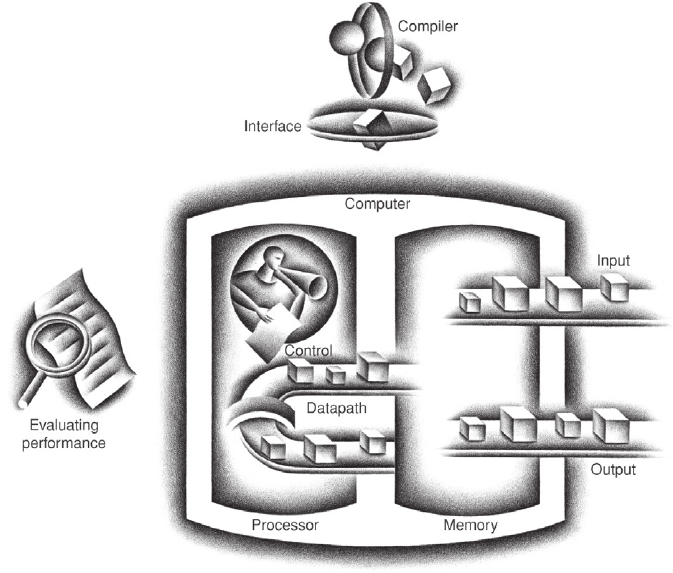
\includegraphics[width=0.65\textwidth, height=0.9\textheight]{docs/images/cpu-high-level}
\end{center}
\end{frame}

\begin{frame}{\lr{Data Path}}
\begin{center}
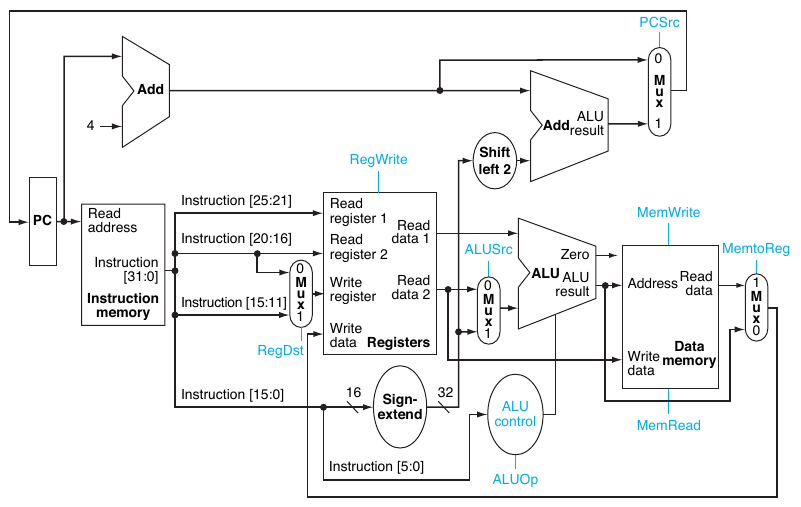
\includegraphics[width=0.85\textwidth, height=0.9\textheight]{docs/images/datapath-clear}
\end{center}
\end{frame}

\begin{frame}{قسمت‌های \lr{Data Path}}
\begin{center}
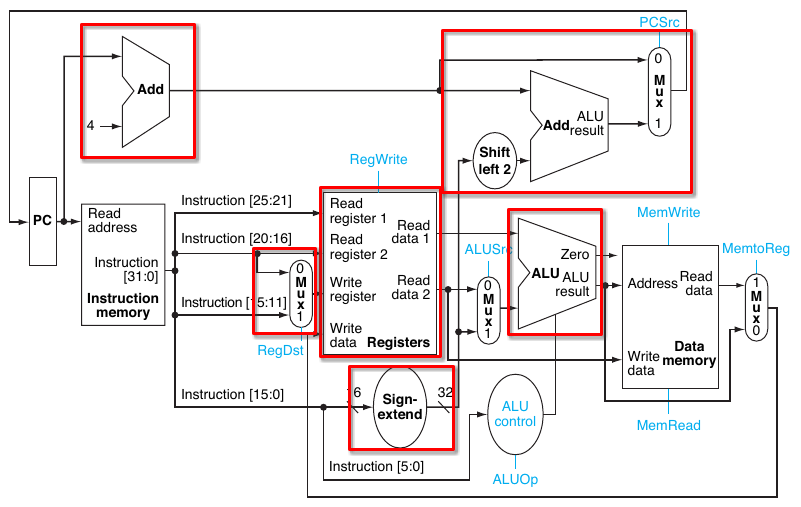
\includegraphics[width=0.85\textwidth, height=0.9\textheight]{docs/images/datapath-parts}
\end{center}
\end{frame}

\begin{frame}{\lr{Control Unit}}
\begin{itemize}\itemr
\item[-]
وقتی برای یک معماری، 
\lr{Instruction Set}
نوشته می‌شود، به این معنی‌ست که هر یک از 
\lr{instruction}
ها یک معنی می‌دهد، یک سری ریجستر خاص را نیاز دارد و باید از مسیر متفاوتی از داخل 
\lr{data path}
رد بشود،
\item[-]
کدگشایی و کنترل کردن مسیر گذر یک 
\lr{instruction}
و داده‌هایش به عهده‌ی 
\lr{Control Unit}
است.
\end{itemize}
\end{frame}

\begin{frame}{\lr{Data Path and Control Unit}}
\begin{center}
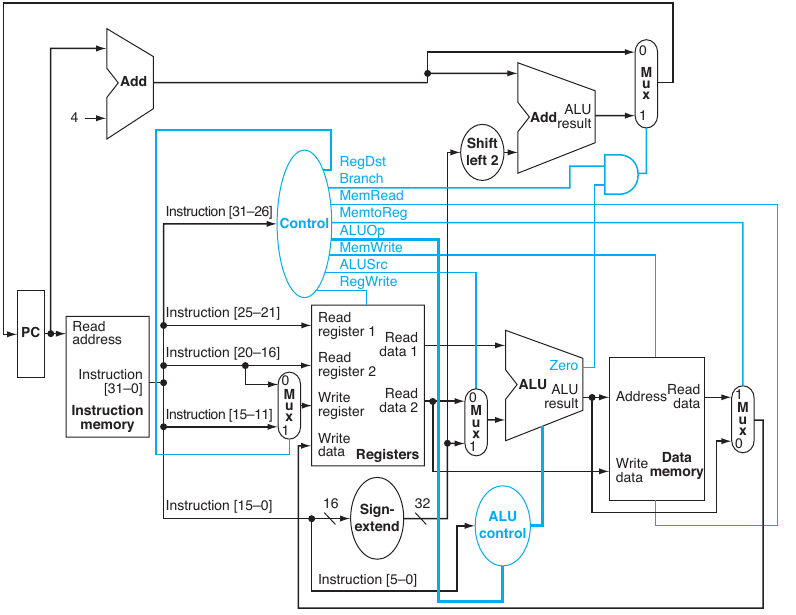
\includegraphics[width=0.65\textwidth, height=0.80\textheight]{docs/images/dp-cu}
\end{center}
\end{frame}

\begin{frame}{\lr{AMD Barcelona Microprocessor}}
\begin{center}
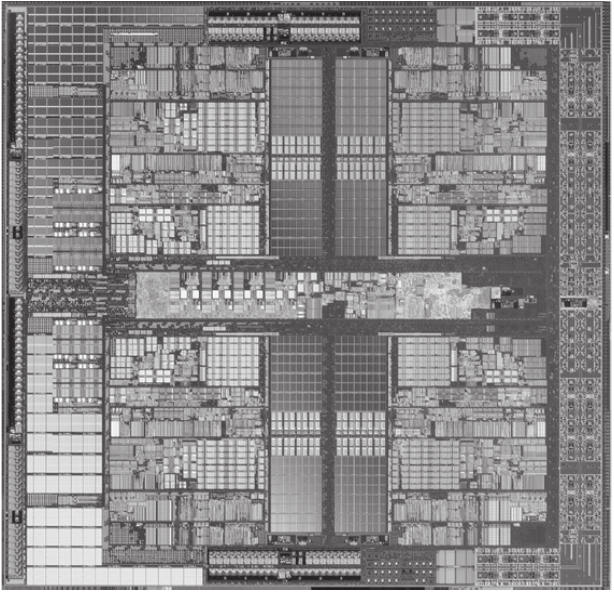
\includegraphics[width=0.50\textwidth, height=0.80\textheight]{docs/images/amd-1}
\end{center}
\end{frame}

\begin{frame}{\lr{AMD Barcelona Microprocessor Sketch}}
\begin{center}
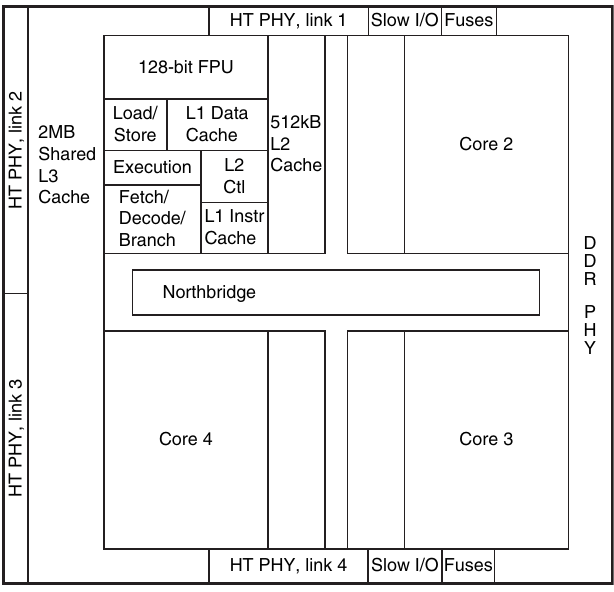
\includegraphics[width=0.5\textwidth, height=0.80\textheight]{docs/images/amd-2}
\end{center}
\end{frame}

\begin{frame}{\lr{AMD Barcelona Microprocessor}}
\begin{center}
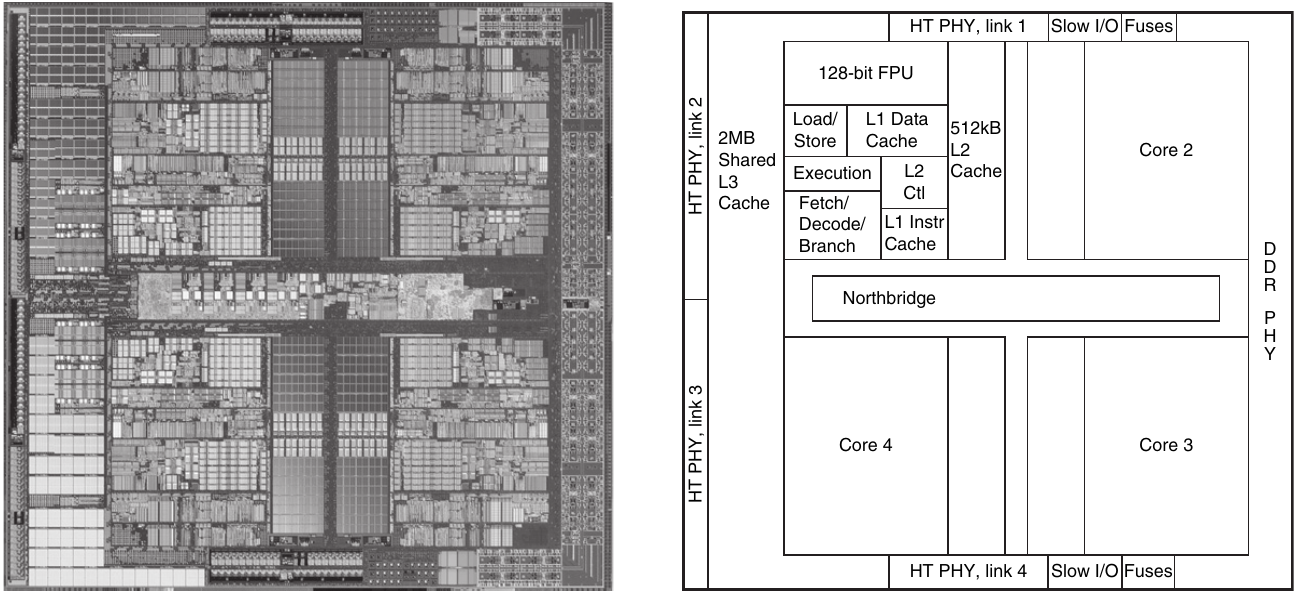
\includegraphics[width=0.9\textwidth, height=0.80\textheight]{docs/images/amd-3}
\end{center}
\end{frame}
